

\documentclass[12pt,AutoFakeBold]{article} 

\usepackage[智能数据挖掘]{XDUreport}  % 科目名称
\problem{DBSCAN 聚类算法练习}  % 请在此处填写问题内容
\labdate{2022 年 05 月 12 日}
% 其他参数在宏包中进行更改,其中学院,班级,姓名,学号均在sty宏包内进行更改
% \usepackage{fourier}  % 这是 fourier 字体,更柔和 

%% 如果你需要中文的一级标题编号,如“一、”、“二、”等,请把下面两行取消注释
% \RequirePackage{zhnumber} % change section number to chinese
% \titleformat{\section}{\Large\bfseries\rmfamily}{\zhnum{section}、}{0em}{}
%\usepackage[table,xcdraw]{xcolor}
%\definecolor{lightblue}{RGB}{222, 234, 246}

% 文档开始
        
\begin{document}

\maketitle
\setcounter{tocdepth}{2}

\tableofcontents  % 生成目录

% 正文标题
\makeatletter
\begin{center}
    \LARGE \textbf{\textsf{\@problem}}
\end{center}
\makeatother

% 正文开始

\section{问题描述}

编程实现 DBSCAN 对如图 \ref{fig:dataSet} 所示数据的聚类。

\begin{figure}[htbp]
	\centering
	\begin{minipage}[t]{0.48\textwidth}
		\centering
		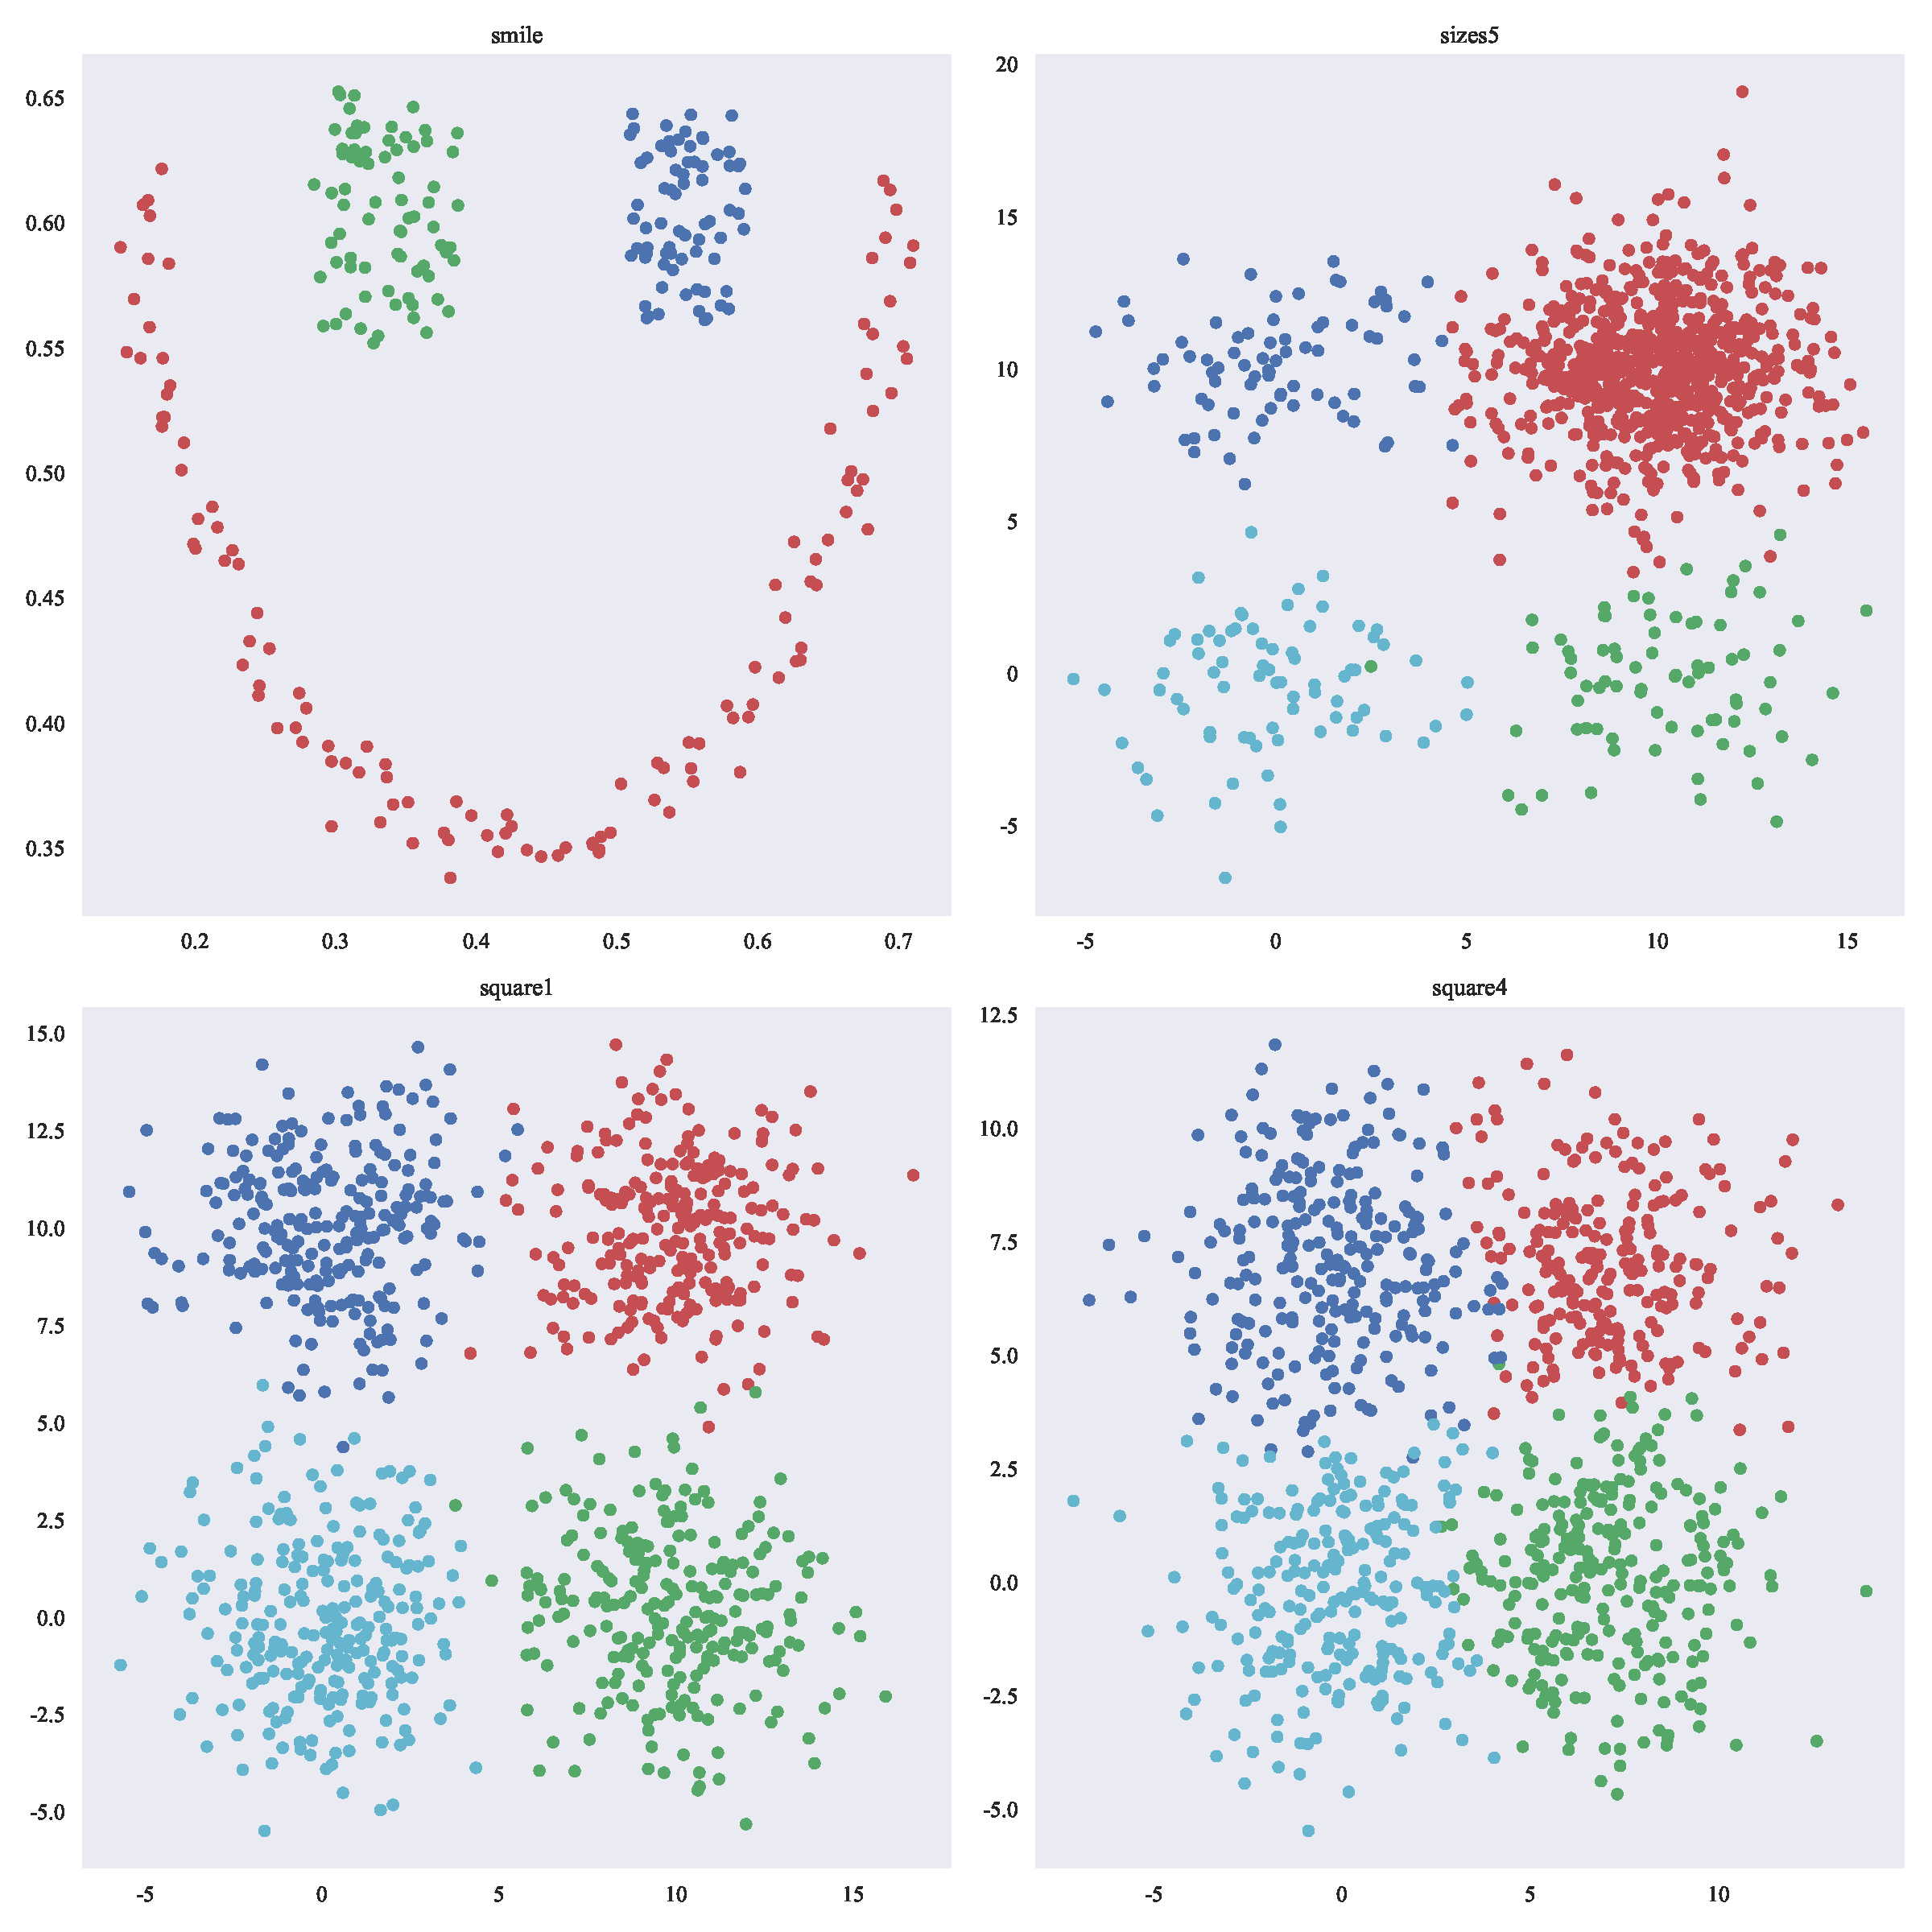
\includegraphics[width=7.5cm]{data1.pdf}
	\end{minipage}
	\begin{minipage}[t]{0.48\textwidth}
		\centering
		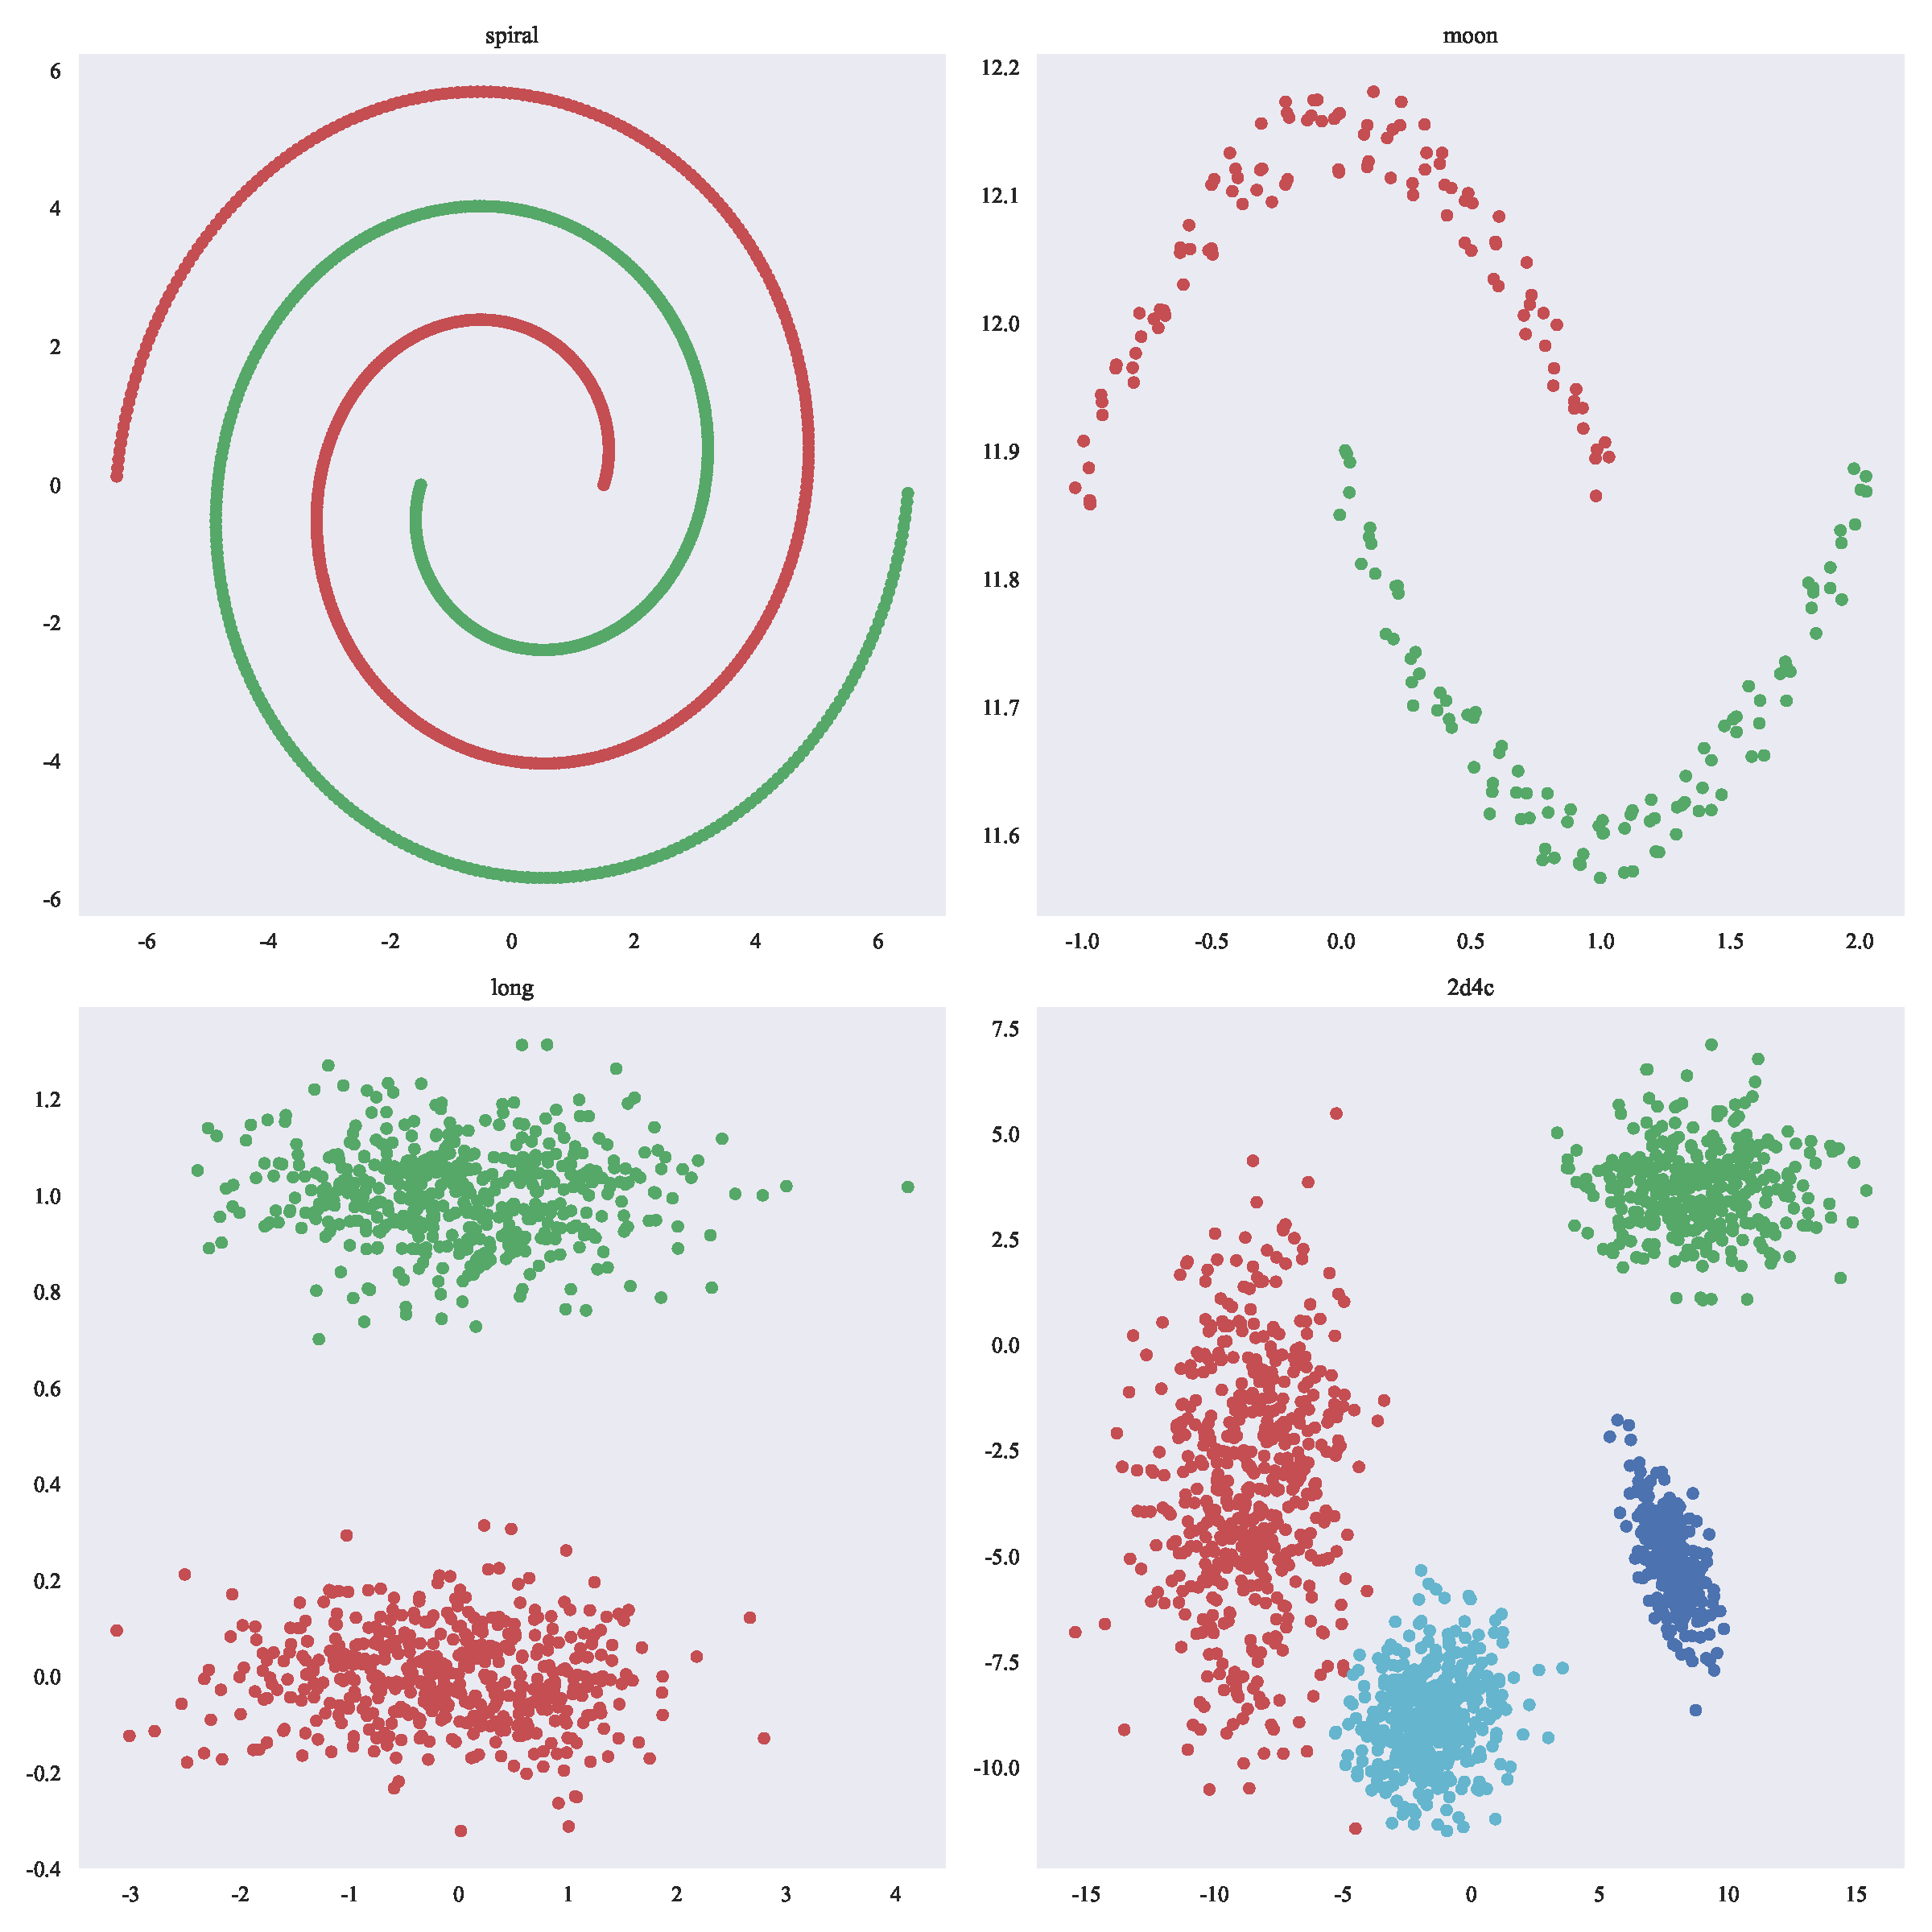
\includegraphics[width=7.5cm]{data2.pdf}
	\end{minipage}
	\caption{数据集展示} \label{fig:dataSet}
\end{figure}

\section{原理分析}

\subsection{DBSCAN 聚类}

DBSCAN (Density-based spatial clustering of applications with noise) 是一种基于密度的聚类算法。与划分和层次聚类方法不同,它将簇定义为密度相连的点的最大集合,能够把具有足够高密度的区域划分为簇。KMeans对于非球状的数据聚类效果不好,但 DBSCAN 可在噪声的空间数据库中发现任意形状的聚类。DBSCAN 基于一组 “领域” (neighborhood) 参数 ($\epsilon, MinPts$) 来刻画样本分布的紧密程度。给定数据集 $D=\{\bm{x}_1,\bm{x}_2,\cdots,\bm{x}_m\}$,定义下面几个概念:

\begin{itemize}
\item $\epsilon$-邻域:对于某一对象点来说,在其半径为 $\epsilon$ 的区域为 $\epsilon$-邻域;
\item 核心对象 (core object):如果一个对象的 $\epsilon$-邻域内至少包含 $MinPts$ 个对象,那么称该对象为核心对象;
\item 密度直达 (directly density-reachable):若 $\bm{x}_j$ 位于 $\bm{x}_i$ 的 $\epsilon$-邻域中,且 $\bm{x}_i$ 是核心对象,则称 $x_j$ 由 $x_i$ 密度直达;
\item 密度可达 (density-reachable):对 $\bm{x}_i$ 和 $\bm{x}_j$,若存在样本序列 $\bm{p}_1,\bm{p}_2,\cdots,\bm{p}_n$,其中 $\bm{p}_1=\bm{x}_i,\bm{p}_n=\bm{x}_j$ 且 $\bm{p}_{i+1}$ 由 $\bm{p}_i$ 密度直达,则称 $\bm{x}_i$ 由 $\bm{x}_j$ 密度可达;
\item 密度相连 (density-connected):对 $\bm{x}_i$ 与 $\bm{x}_j$,若存在 $\bm{x}_k$ 使得 $\bm{x}_i$ 与 $\bm{x}_j$ 均由 $\bm{x}_k$ 密度可达,则称 $\bm{x}_i$ 与 $\bm{x}_j$ 密度相连;
\item 噪声 (noise):与任何点都不可达的对象称为噪声。
\end{itemize}

DBSCAN 聚类伪代码如算法 \ref{alg:DBSCAN} 所示。

%\begin{figure}[htb]
%\centering
%\begin{minipage}{.8\linewidth}
\begin{algorithm}[H]
	\caption{DBSCAN 聚类}
	\label{alg:DBSCAN}
	\begin{algorithmic}[1]
	\Require 样本集 $D=\{\bm{x}_1,\bm{x}_2,\cdots,\bm{x}_m\}$; 邻域参数 $(\epsilon, MinPts)$.
	\Ensure 簇划分 $\mathcal{C} = \{C_1,C_2,\cdots,C_k\}$.
	
	\State 初始化核心对象集合:$\Omega=\oslash$;
	\For {$j=1,2,\cdots,m$}
		\State 确定样本 $\bm{x}_j$ 的 $\epsilon$-邻域 $N_\epsilon(\bm{x}_j)$;
		\If {$N_\epsilon(\bm{x}_j)\ge MinPts$}
			\State 将样本 $\bm{x}_j$ 加入核心对象集合: $\Omega=\Omega\bigcup\{\bm{x_j}\}$;
		\EndIf
	\EndFor
	\State 初始化聚类簇数: $k=0$;
	\State 初始化未访问样本集合: $\Gamma=D$;
	\While {$\Omega\neq\oslash$}
		\State 记录当前未访问样本集合: $\Gamma_{\mathrm{old}}=\Gamma$;
		\State 随机选取一个核心对象 $\bm{o}\in\Omega$,初始化队列 $Q=<\bm{o}>$;
		\State $\Gamma=\Gamma\backslash\{\bm{o}\}$;
		\While {$Q\neq\oslash$}
			\State 取出队列 $Q$ 中的首个样本 $\bm{q}$;
			\If {$N_\epsilon(\bm{q})\ge MinPts$}
				\State 令 $\Delta=N_\epsilon(\bm{q})\bigcap\Gamma$;
				\State 将 $\Delta$ 中的样本加入队列 $Q$;
				\State $\Gamma=\Gamma\backslash\Delta$;
			\EndIf
		\EndWhile
		\State $k=k+1$, 生成聚类簇 $C_k=\Gamma_{\mathrm{old}}\backslash\Gamma$;
		\State $\Omega=\Omega\backslash C_k$;
	\EndWhile
	\end{algorithmic} 
\end{algorithm}
%\end{minipage}
%\end{figure}

\section{实验过程}

\subsection{算法实现}

实现 DBSCAN 聚类算法步骤如下,具体代码见附录。

\begin{enumerate}
\renewcommand{\labelenumi}{\bfseries \textit{Step} \theenumi.}

\item 任意选择一个未访问过的点 P。

\item 标记点 P 为已访问。

\item 计算得到所有从 P 关于 Eps 和 MinPts 密度可达的点的集合 NeighborPts。

\item 若 P 不是核心对象,标记点 P 为噪声,跳转步骤 S1 重新选取 P;若 P 为核心对象,则扩展当前核心对象 P 的所属簇 (expandCluster 函数)。

\item 判断是否所有点均已被访问,若是则跳转 \textbf{\textit{Step} 6}; 若否则继续 \textbf{\textit{Step} 1$\sim$5} 步骤。

\item DBSCAN 算法运行结束,返回 Cluster 分类数组。
\end{enumerate}

%\subsection{8 个数据集上应用}
\subsection{smile 数据集}

设置 Eps=0.05,MinPts=3,使用 DBSCAN 聚类得到如图 \ref{fig:smile} 所示的结果。

\begin{figure}[H]
	\centering
    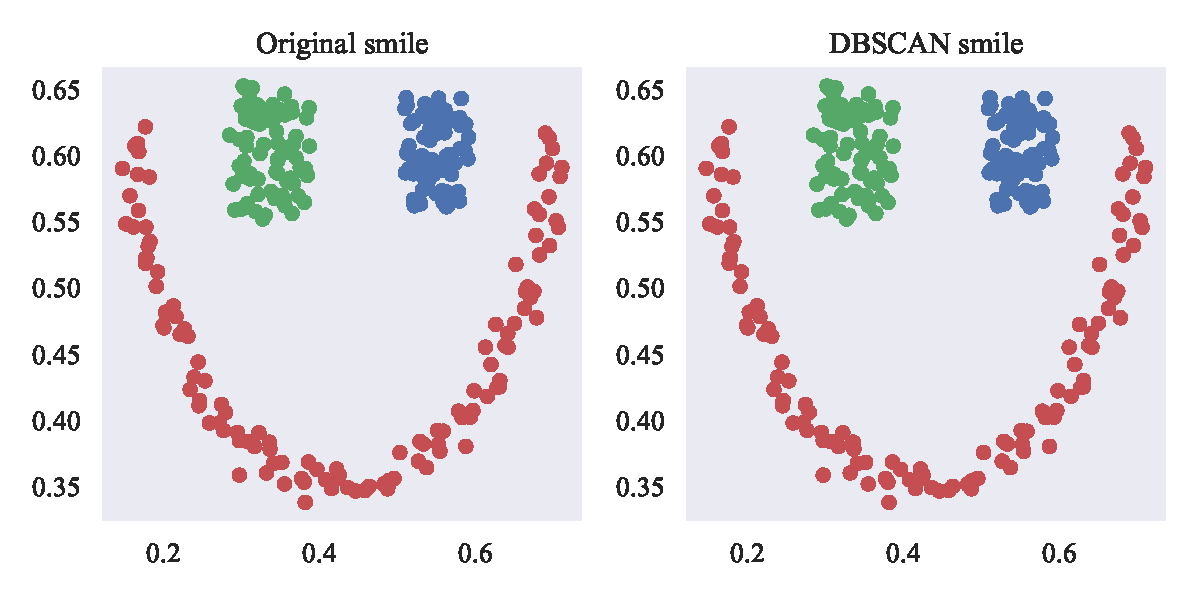
\includegraphics[width=0.7\textwidth]{smile.pdf}
    \caption{DBSCAN 对 smile 数据集聚类结果} \label{fig:smile}
\end{figure}

\subsection{sizes5 数据集}

设置 Eps=1,MinPts=3,使用 DBSCAN 聚类得到如图 \ref{fig:sizes5} 所示的结果。

\begin{figure}[H]
	\centering
    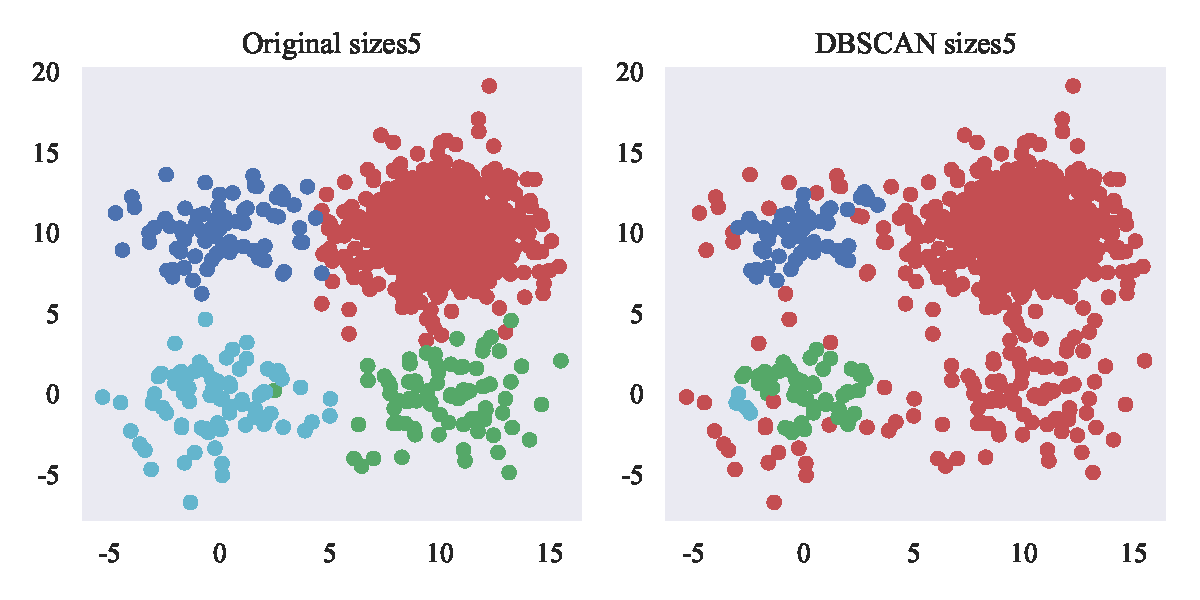
\includegraphics[width=0.7\textwidth]{sizes5.pdf}
    \caption{DBSCAN 对 sizes5 数据集聚类结果} \label{fig:sizes5}
\end{figure}

\subsection{square1 数据集}

设置 Eps=1,MinPts=5,使用 DBSCAN 聚类得到如图 \ref{fig:square1} 所示的结果。

\begin{figure}[H]
	\centering
    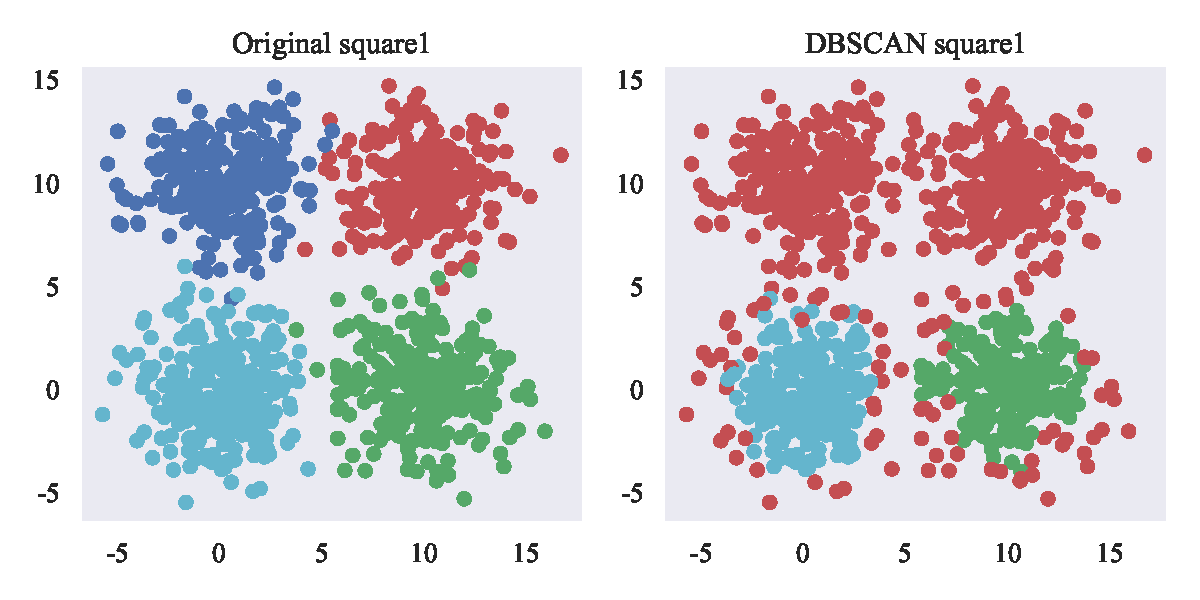
\includegraphics[width=0.7\textwidth]{square1.pdf}
    \caption{DBSCAN 对 square1 数据集聚类结果} \label{fig:square1}
\end{figure}

\subsection{square4 数据集}

设置 Eps=1,MinPts=3,使用 DBSCAN 聚类得到如图 \ref{fig:square4} 所示的结果。

\begin{figure}[H]
	\centering
    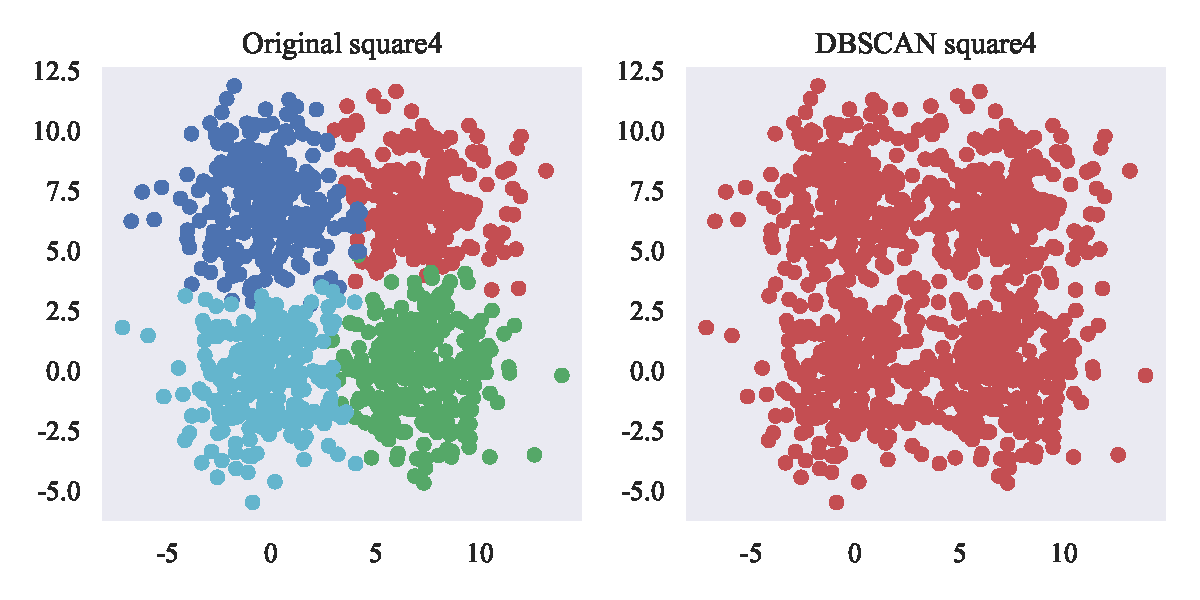
\includegraphics[width=0.7\textwidth]{square4.pdf}
    \caption{DBSCAN 对 square4 数据集聚类结果} \label{fig:square4}
\end{figure}

\subsection{spiral 数据集}

设置 Eps=1,MinPts=5,使用 DBSCAN 聚类得到如图 \ref{fig:spiral} 所示的结果。

\begin{figure}[H]
	\centering
    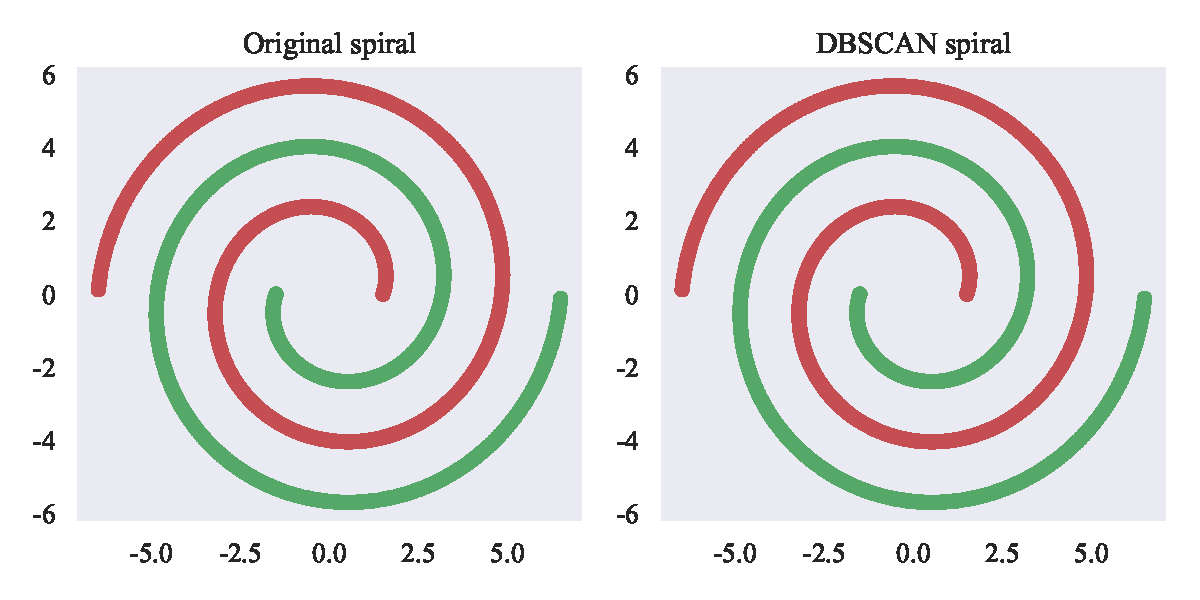
\includegraphics[width=0.7\textwidth]{spiral.pdf}
    \caption{DBSCAN 对 spiral 数据集聚类结果} \label{fig:spiral}
\end{figure}

\subsection{moon 数据集}

设置 Eps=0.2,MinPts=5,使用 DBSCAN 聚类得到如图 \ref{fig:moon} 所示的结果。

\begin{figure}[H]
	\centering
    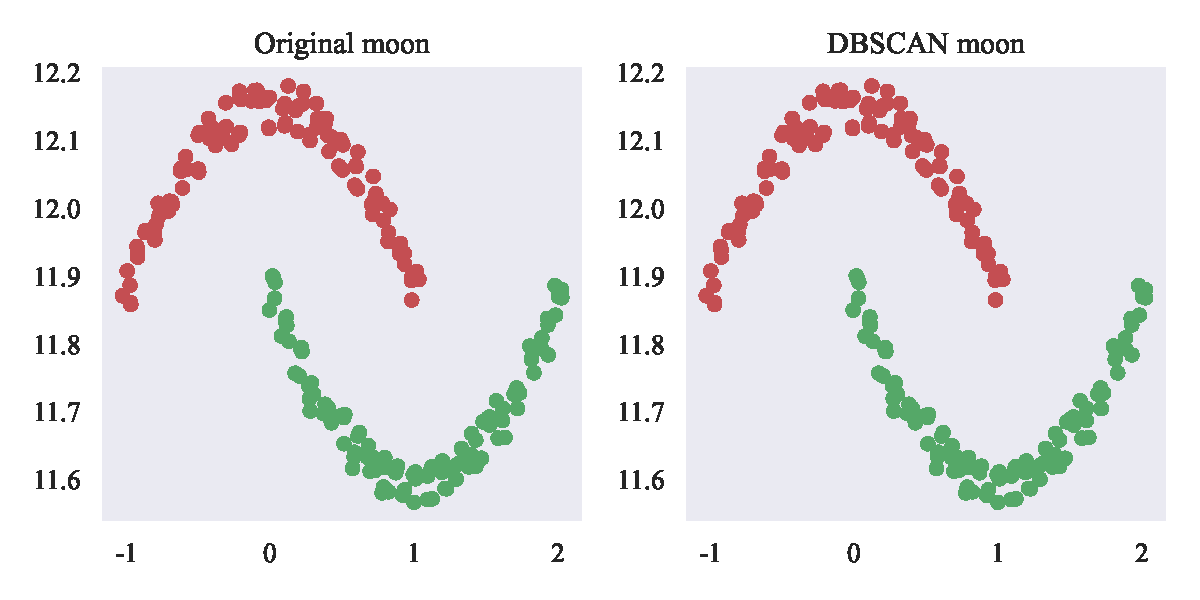
\includegraphics[width=0.7\textwidth]{moon.pdf}
    \caption{DBSCAN 对 moon 数据集聚类结果} \label{fig:moon}
\end{figure}

\subsection{long 数据集}

设置 Eps=0.2,MinPts=5,使用 DBSCAN 聚类得到如图 \ref{fig:long} 所示的结果。

\begin{figure}[H]
	\centering
    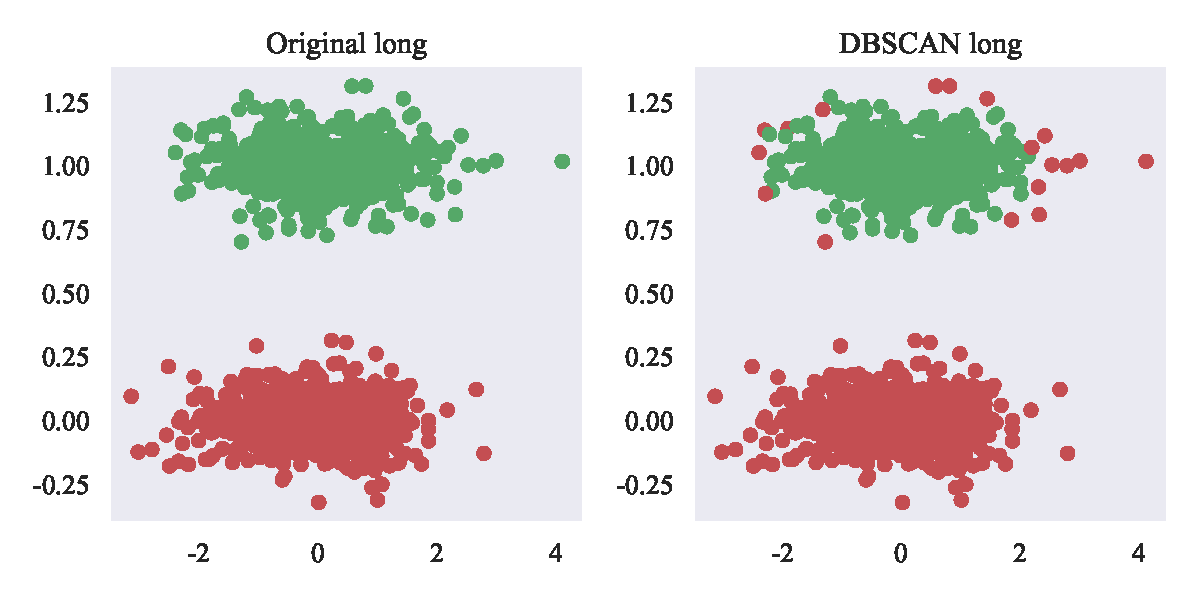
\includegraphics[width=0.7\textwidth]{long.pdf}
    \caption{DBSCAN 对 long 数据集聚类结果} \label{fig:long}
\end{figure}

\subsection{2d4c 数据集}

设置 Eps=0.5,MinPts=5,使用 DBSCAN 聚类得到如图 \ref{fig:2d4c} 所示的结果。

\begin{figure}[H]
	\centering
    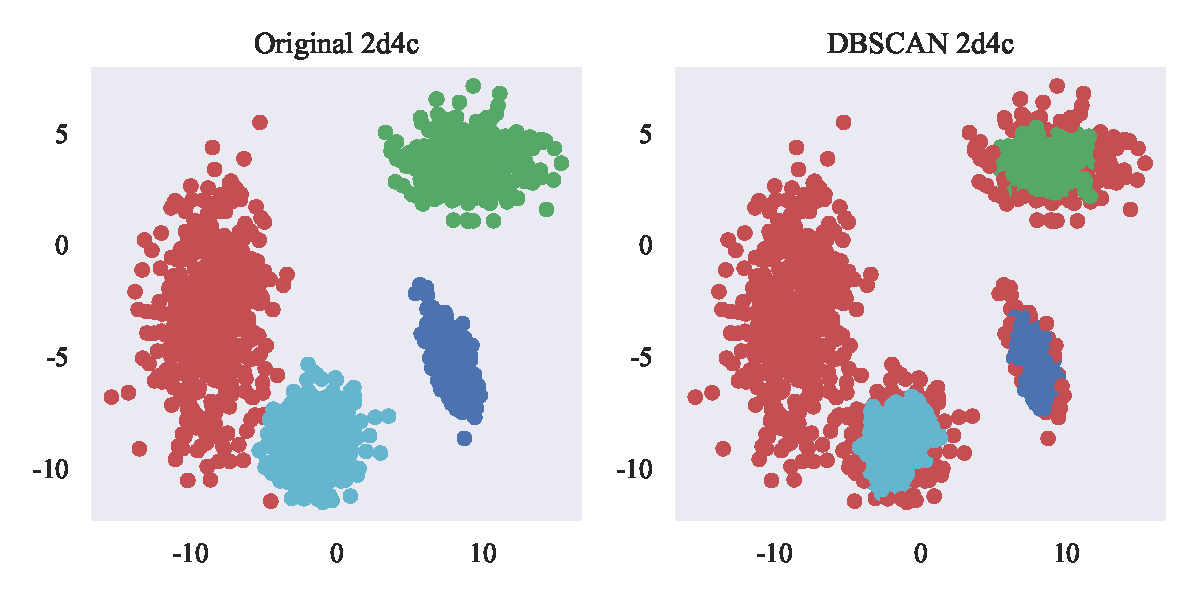
\includegraphics[width=0.7\textwidth]{c4d2.pdf}
    \caption{DBSCAN 对 2d4c 数据集聚类结果} \label{fig:2d4c}
\end{figure}

\newpage

\includepdfset{pagecommand={\thispagestyle{fancy}}} 
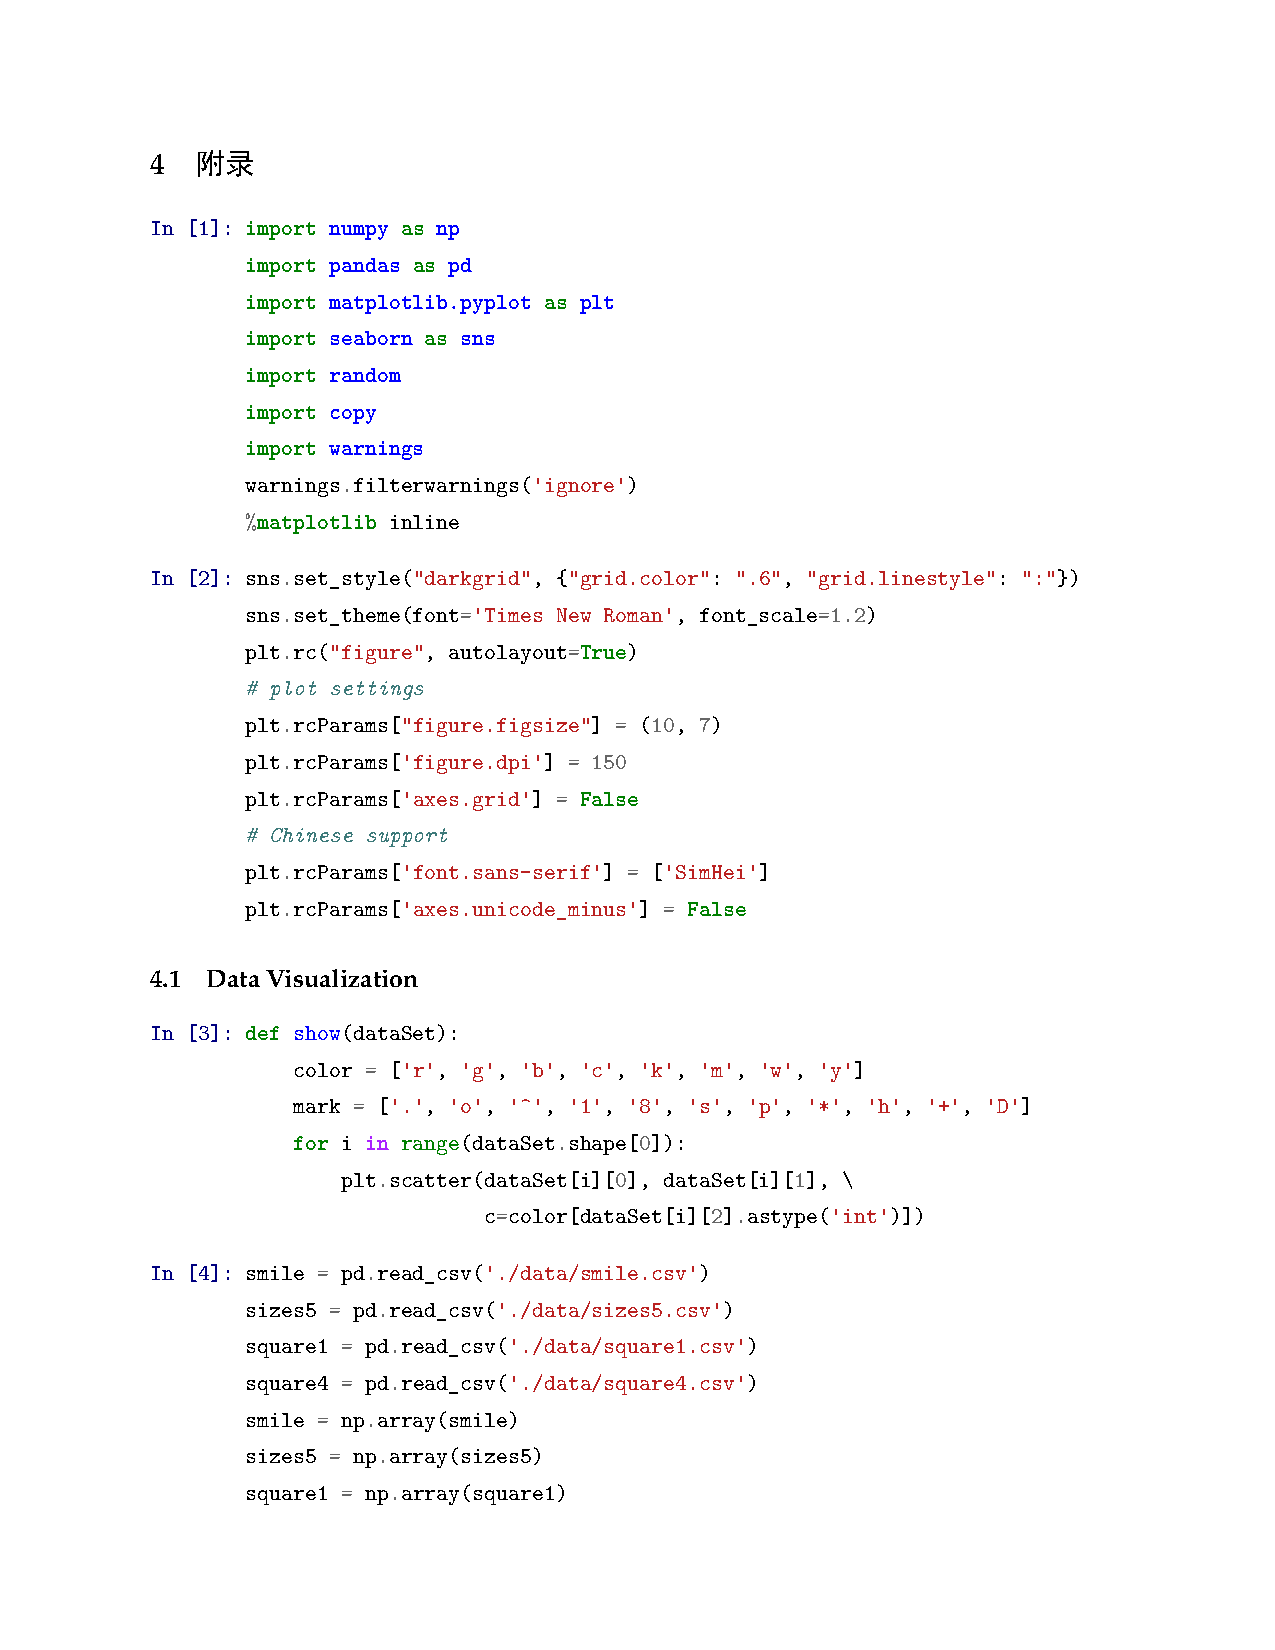
\includepdf[addtotoc={1,section,1,附录,appendix}, pages={1-14}]{DBSCAN.pdf}

% % 参考文献,此处以 MLA 引用格式为例

% \begin{thebibliography}{9}
%     \bibitem{1} Clemente, Filipe Manuel, et al. "General network analysis of national soccer teams in FIFA World Cup 2014." \emph{International Journal of Performance Analysis in Sport} 15.1 (2015): 80-96.
%     \bibitem{3} Dijkstra, Edsger Wybe. "A Note on Two Problems in Connexion With Graphs." \emph{Numerische Mathematik} 1(1959):269-271.
%     \bibitem{4} Ahnert, Sebastian E., et al. "Ensemble approach to the analysis of weighted networks.." \emph{Physical Review E} 76.1 (2007).
%     \bibitem{5} Wong, J. A. Hartiganm. A. . "Algorithm AS 136: A K-Means Clustering Algorithm." \emph{Journal of the Royal Statistical Society. Series C (Applied Statistics)} 28.1(1979):100-108.
%     \bibitem{6} Buldu, J. M., et al. "Defining a historic football team: Using Network Science to analyze Guardiola’s F.C. Barcelona." \emph{Scientific Reports} 9.1 (2019): 1-14.
%     \bibitem{7} \emph{Balotelli sends Italy past Germany}. (2012). Retrieved December 10, 2014, from\url{https://www.uefa.com/uefaeuro/season=2012/matches/round=15174/match=2003379/index.html}
%     \bibitem{8} Sigari, Mohamad Hoseyn, et al. "Counterattack detection in broadcast soccer videos using camera motion estimation." \emph{international symposium on artificial intelligence} (2015): 101-106.
%     \bibitem{9} Abdelmahmoud Hassan Elsheikh. \emph{Effect of Leadership Intensity on Integrating Some Formal and Informal Organizational Efforts for Community Development in Khartoum Province}. 2016.
% \end{thebibliography}


% \includepdf[pages={1,2}]{Memo.pdf} 
% 可以直接导入pdf页面
% \newpage
% \begin{appendices}  % 附录环境
% \section{附录}
% \end{appendices}

\end{document}  % 结束